\documentclass{article}

\usepackage{amssymb}
\usepackage{amsmath}
\usepackage{fontspec}
\usepackage{setspace}
\setmainfont{Cambria}
\usepackage[margin=0.5in]{geometry}
\usepackage{tikz}
\usepackage{tkz-euclide}
\usetkzobj{all}
\usepackage{multicol}

\DeclareMathOperator{\re}{Re}
\DeclareMathOperator{\im}{Im}

\begin{document}
\begin{center}
\begin{huge}
TAIU10 Sammanfattning

\end{huge}
\end{center}
\section{Reella och Komplexa Tal}
Intervall med oändlighet är alltid öppna, ex. $[x, \infty[$ eller $]-\infty, x[$\\

\setcounter{subsection}{1}
\subsection{Algebraisk räkning med reella tal}
\textbf{Kvadratregeln}: $(a + b)^{2} = a^{2} + 2ab + b^{2}$\\
\textbf{Konjuratregeln}: $(a + b)(a - b) = a^{2} - b^{2}$\\
\textbf{Kubregeln}: $(a + b)^{3} = a^{3} + 3a^{2}b + 3ab^{2} + b^3$\\

\subsection{Ekvationer, koordinatsystem och räta linjer}
\boldmath{$ab = ac \Rightarrow a = 0 \vee b = c$} Lösningen $a = 0$ missas lätt om a divideras bort från båda sidor.\\
\\
Koordinatsystem delas upp i kvadranter enligt
$\begin{array}{c|c}
2 & 1 \\
\hline
3 & 4 \\
\end{array}$\\
\\
En rät linje med punkterna $P_1 = (x_1, y_1)$ och $P_2 = (x_2, y_2), P_1 \neq P_2$ har en riktningskoefficient $k$  med formeln $k = \dfrac{y_2 - y_1}{x_2 - x_1}$. En generell ekvation för en linje med en känd punkt och känd riktningskoeffecient ges av $y = y_1 + k(x - x_1)$, också kallad \textbf{enpunksformeln}.

\subsection{Mer om ekvationer}
\underline{En} lösning finns för $x = \sqrt{a}, x^2$\\
\underline{Två} lösningar finns för $x^2 = a, x = \sqrt(a)$ och $x = -\sqrt(a)$

\subsubsection{Generell kvadratkomplettering}
$x^2 + ax + b = 0 \Leftrightarrow  (x + \dfrac{a}{2})^2 - (\dfrac{a}{2})^2 + b = 0 \Leftrightarrow (x + \dfrac{a}{2})^2 = (\dfrac{a}{2})^2 - b \Leftrightarrow x + \dfrac{a}{2} = \pm \sqrt{(\dfrac{a}{2})^2 - b} \Leftrightarrow x = -\dfrac{a}{2} \pm \sqrt{(\dfrac{a}{2})^2 - b} $

\subsubsection{Avstånd och cirklar}
\textbf{Avståndsformeln}: $\sqrt{(x_2 - x_1)^2 + (y_2 - y_1)^2} $

\subsubsection {n-te rötter}
n-te roten av $a$ skrivs $\sqrt[n]{a}$\\
För \underline{jämna} tal $n$ finns \underline{två} reella lösningar till ekvationen $x^n = a, x = a$ samt $x = -a$.\\
För \underline{udda} tal $n$ finns \underline{en} reell lösning till ekvationen $x^n = a, x = a$.\\

\subsubsection{Division av ekvationer}
Om en ekvation $f(x)$ har en rot $c$, kan ekvationen $f(x)$  jämnt delas sådant att $f(x) = (x - c)q(x)$.

\subsection{Olikheter och absolutbelopp}
Då man multiplicerar eller dividerar med en olikhet vänds olikheten: $a > b \Leftrightarrow -a < -b$

\subsection{Summor och Produkter}
\textbf{Aritmetisk summa} $a_m + a_{m+1} + ... + a_n = \sum\limits_{k = m}^n a_k$ sådan att differensen $a_{k+1} - a_k = x$ för alla tal $k = m, ..., n-1$, formel: $a_m + a_{m+1} + ... + a_n = (n  - m + 1) \cdot \dfrac{a_m + a_n}{2}$ \\
\textbf{Geometrisk summa} $a + aq + aq^2 + ... + aq^n = \sum\limits_{k = 0}^n aq^k$ har första termen $a$ och samma kvot $q$ mellan varje term och föregående term. Formel: $a + aq + aq^2 + ... + aq^n = \dfrac{a(q^{n+1} - 1))}{q - 1}$ där $a$ är första termen och $n + 1$ är antal termer.

\subsection{Binomialkoefficienter}
\textbf{Binomialformeln}: $(a + b)^n = \sum\limits_{k=0}^n \binom{n}{k}a^{n-k}b^k$\\
$\binom{n}{k} = \dfrac{n!}{k!(n-k)!}$\\
\\
$\binom{n}{k} = \binom{n}{n-k}$
\subsection{Komplexa tal}
\subsubsection{Allmäna identiteter}

\begin{doublespace}
$z = x + iy$ \\ $i^2 = i \cdot i = -1$ \\ $i = \sqrt{-1}$ \\ $\re(z) = x$ \\ $\im(z) = y$ \\
$z_1 - z_2 = x_1 - x_2 + i(y_1 - y_2)$ \\
$|z| = \sqrt{x^2 + y^2}$ \\
$\bar{z} = x - iy$ \\
$z\bar{z} = |z|^2$ \\
$|z_1 + z_2| \leq |z_1| + z_2|$ \\
För att underlätta division av komplexa tal, kan man förlänga med nämnarens konjugat:\\
$\dfrac{z_1}{z_2} = \dfrac{z_1\bar{z_2}}{z_2\bar{z_2}} = \dfrac{z_1\bar{z_2}}{|z_2|^2}$ \\
Detta gör att nämnaren blir reell.
\end{doublespace}
\subsection{Funktioner}
\subsubsection{Definitions-och värdemängd, invers}
$D_f$ är definitionsmängden för $f(x)$, d.v.s vilka värden $x$ kan anta.\\
$V_f$ är värdemängden för $f(x)$, d.v.s. de värden $f(x)$ kan anta. \\
En funktion är jämn om $f(x) = f(-x)$. En funktion är ojämn om $f(-x) = -f(x)$.
\\
En funktion är omvändbar om det för varje $y \in D_f$ finns exakt ett $x \in D_f$ sådant att $f(x) = y$. Inversen betecknas då $f^{-1}$, $f(x) = y \Leftrightarrow f^{-1}(y) = x$.
\subsubsection{Växande, avtagande, begräsning}
En funktion är växande om den för varje $x_2 > x_1 \Rightarrow f(x_2) \geq f(x_1)$. Omvänt är funktionen avtagande om det för varje $x_2 > x_1 \Rightarrow f(x_2) \leq f(x_1)$.\\
En funktion är strängt avtagande om $x_2 > x_1 \Rightarrow f(x_2) > f(x_1)$, och omvänt för strängt avtagande.\\
En funktion är begränsad ifall alla $y \in V_f$ är mindre eller större än något reellt tal $a$. Exempelvis är $x^2$ begränsad nedåt, då $x^2 \geq 0$.
\section{Naturliga logaritmen, exponential- och potensfunktioner}
$ln$ har definitionsmängden $D_{ln} = ]0,\infty[ och V_{ln} = \mathbb{R}$
\subsubsection{Räkneregler}
\begin{doublespace}
$\ln(xy) = \ln x + \ln y$\\
$\ln(1) = 0$\\
$\ln(\dfrac{x}{y}) = \ln(x) - \ln(y)$ \\
$\ln(\dfrac{1}{x} = -\ln(x)$\\
$\ln(x^p) = p \cdot ln x$\\
$\ln$ är strängt växande, d.v.s. $x_1 > x_2 \Rightarrow \ln(x_1) > \ln(x_2)$\\
$\ln x$ = $\left\{
    \begin{array}{l}
      A_x$ för $x \geq 1 \\
      -A_x$ för $0 < x < 1 \\
    \end{array}\right.$\\[10pt]
\end{doublespace}
\subsection{Exponentialekvationer och talet e}
\begin{doublespace}
$\ln^{-1}$ kallas den naturliga exponentialekvationen.\\
$y = \exp(x) \Leftrightarrow x = \ln(y)$\\
$D_{\exp} = V_{ln} = \mathbb{R}$ \\
$e = \exp(1)$\\
$a^x = e^{x\cdot \ln(a)}$
\subsection{Allmäna logaritmfunktionen}
$y = \log_a(x) \Leftrightarrow x = a^y$\\
$y = \log_a(x) = \dfrac{\ln(x)}{\ln(a)}$ för alla $x > 0$\\
\end{doublespace}
\section{Trigonometri}
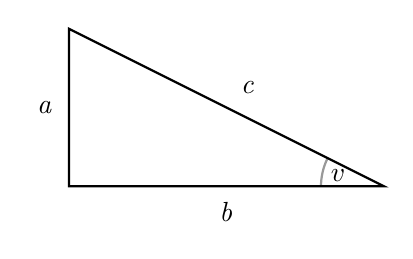
\begin{tikzpicture}[thick]
\coordinate (O) at (0,0);
\coordinate (A) at (4,0);
\coordinate (B) at (0,2);
\draw (O)--(A)--(B)--cycle;

\tkzLabelSegment[below=2pt](O,A){\textit{b}}
\tkzLabelSegment[left=2pt](O,B){\textit{a}}
\tkzLabelSegment[above right=2pt](A,B){\textit{c}}

\tkzMarkAngle[size=0.8cm,%
opacity=.4](B,A,O)
\tkzLabelAngle[pos = 0.6](B,A,O){$v$}
\end{tikzpicture}\\
\begin{doublespace}
$cos v = \dfrac{b}{c}$\\
$sin v = \dfrac{a}{c}$\\
$tan v = \dfrac{a}{b}$\\
$cot v = \dfrac{b}{a}$\\
\end{doublespace}
\subsubsection{Värden för vanliga vinklar}
\begin{tabular}{c|c|c|c|c}
v & cos v & sin v & tan v & cot v \\
\hline
$\dfrac{\pi}{6}$ & $\dfrac{\sqrt{3}}{2}$ & $\dfrac{1}{2}$ & $\dfrac{1}{\sqrt{3}}$  & $\sqrt{3}$\\
\hline
$\dfrac{\pi}{4}$ & $\dfrac{1}{\sqrt{2}}$ & $\dfrac{1}{\sqrt{2}}$ & 1 & 1\\
\hline
$\dfrac{\pi}{3}$ & $\dfrac{1}{2}$ & $\dfrac{\sqrt{3}}{2}$ & $\sqrt{3}$ & $\dfrac{1}{\sqrt{3}}$
\end{tabular}
\subsubsection{Räkneregler}
\begin{doublespace}
\begin{minipage}[t]{0.5\textwidth}
$\cos^2 v + \sin^2 v = 1\\
\cos -v = cos v\\
\sin -v = -\sin v\\
\tan -v = -\tan v\\
\cot -v = -\tan v\\
\\
\cos(\pi - v) = -\cos v\\
\sin(\pi - v) = \sin v\\
\\
\cos(\dfrac{\pi}{2} - v) = \sin v\\
\sin(\dfrac{\pi}{2} - v) = \cos v\\
$
\end{minipage}
\begin{minipage}[t]{0.5\textwidth}
$\cos(v + 2\pi) = \cos v\\
\sin(v + 2\pi) = \sin v\\
\\
\cos(v + \pi) = -\cos v\\
\sin(v + \pi) = -\sin v\\
\tan(v + \pi) = \tan v\\
\cot(v + \pi) = \cot v\\
\\
\cos(u+v) = \cos u \sin v - \cos v \sin u\\
\cos(u-v) = \cos u \sin v + \cos v \sin u\\
\sin(u+v) = \sin u \cos v + \sin v \cos u\\
\sin(u-v) = \sin u \cos v - \sin v \cos u\\
\tan(u+v) = \dfrac{\tan u + \tan v}{1 - \tan u \tan v}\\
$
\end{minipage}
$\cos 2v = \cos^2 v - \sin^2 v = 2\cos^2 v - 1= 1 - 2\sin^2 v$\\
$\sin 2v = 2\sin v \cos v$\\
$\tan 2v = \dfrac{2\tan v}{1 - \tan^2 v}$\\
\\
$\dfrac{1}{\cos^2 v} = 1 + \tan^2 v$\\
$|\sin v| \leq |v|$ för $v \in \mathbb{R}$\\
$\cos u + \cos v = 2\cos \dfrac{u+v}{2} \cos \dfrac{u-v}{2}$\\
$\cos u - \cos v = -2\sin \dfrac{u+v}{2} \sin \dfrac{u-v}{2}$\\
$\sin u + \sin v = 2\sin \dfrac{u+v}{2} \cos \dfrac{u-v}{2}$\\
$\sin u - \sin v = 2\cos \dfrac{u+v}{2} \sin \dfrac{u-v}{2}$\\
\end{doublespace}
\subsection{Den komplexa exponentialfunktionen}
\begin{doublespace}
$e^{ix} = \cos x + i \sin x$ för $x \in \mathbb{R}$\\
\begin{minipage}[t]{0.5\textwidth}
$\cos x = \dfrac{e^{ix} + e^{-ix}}{2}$\\
\end{minipage}
\begin{minipage}[t]{0.5\textwidth}
$\sin x = \dfrac{e^{ix} - e^{-ix}}{2i}$\\
\end{minipage}
$|e^{ix}| = 1$
\subsubsection{Komplexa tal i polär form}
\begin{minipage}[t]{0.5\textwidth}
$x = r \cos x$
\end{minipage}
\begin{minipage}[t]{0.5\textwidth}
$y = r \sin v$
\end{minipage}
$z = r(\cos v + i \sin v) = re^{iv}$\\
$e^z = e^{x + iy} = e^xe^{iy} = e^x(\cos y + i\sin y)$\\
$r = |z| = \sqrt{x^2 + y^2}$\\
\textbf{de Moivres formel}: $z^p = r^pe^{ipv} = r^p(\cos pv + i\sin pv)$
\end{doublespace}
\end{document}